\documentclass[a4paper,titlepage]{scrartcl}
\pagestyle{plain}
\usepackage[utf8]{inputenc}
\usepackage[T1]{fontenc}
\usepackage[german]{babel}
\usepackage{units}
\usepackage{floatrow}
\usepackage{amsmath,amssymb,amstext}
\usepackage{pgfplots,pgfplotstable}
\usepackage{numprint}
\usepackage{graphicx}

\newfloatcommand{capbtabbox}{table}[][\FBwidth]
\numberwithin{equation}{section}

\title{Auswertung vom Versuch P2-72: Gamma-Spektroskopie und Statistik}
\author{Gruppe Di-22\\Genti Saliu}
\date{16. Juli 2014}

\begin{document}

\begin{titlepage}
\maketitle
\thispagestyle{empty}
\end{titlepage}

\newpage
\pagenumbering{roman}
\tableofcontents

\newpage
\pagenumbering{arabic}

\section{Aufnahme von Impulshöhenspektren}
Es sollten in diesem Versuch die Impulshöhenspektren der Gamma-Strahlung verschiedener Teilchen aufgenommen und diese bzw. ihre Energien gedeutet werden. Das Impulshöhenspektrum ist die Anzahl der Ereignisse in Abhängigkeit von der Energie der Gamma-Strahlen.
\subsection{Impulshöhenspektren der $\gamma$-Strahlung vom Untergrund, Cs-137, Na-22 und Co-60 mit dem 1024-Kanalbetrieb}
Zunächst wurde das Untergrundspektrum ohne Probe aufgenommen um dessen Einfluss auf unsere Messung zu überprüfen. Wir stellten CASSY in 1024-Kanalbetrieb ein und führten Messungen über einen Zeitraum von $\unit[300]{s}$ durch. Es wurde zudem eine Anpassung der Beschleunigungsspannung am Szintillator vorgenommen, damit das Photopeak möglichst am rechten Rand zu sehen war.
\begin{figure}[H]
		\centering
		\begin{tabular}{@{}r@{}}
			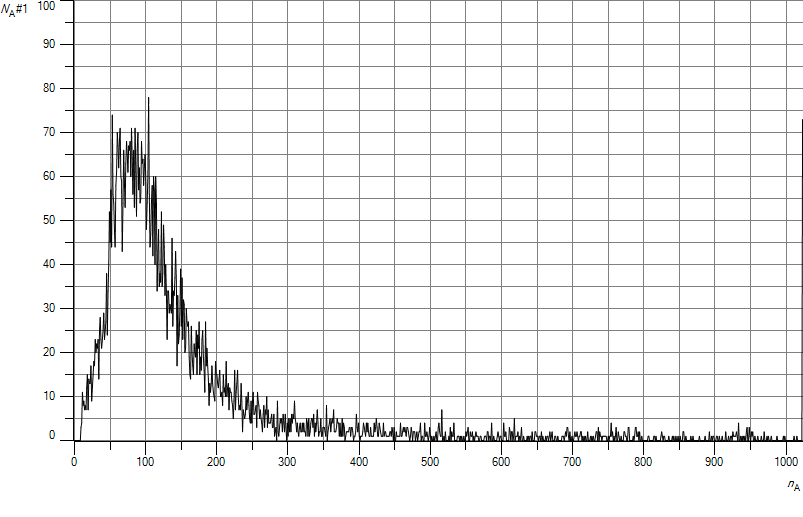
\includegraphics[width=0.8\textwidth]{bilder/aufgabe1/untegrundspektrum.png}\\
		\end{tabular}
		\caption{Impulshöhenspektrum vom Untergrund}
\end{figure}
Die Zählrate der Untergrundstrahlung wurde im Labor nicht festgehalten, diese konnte ich bei der Auswertung aus den CASSY-Messdaten anhand des Durchschnitts aller gespeicherten Zählraten bestimmen und fand $R_A=\unit[29.35]{\frac{1}{s}}$. Verglichen mit den zu erwartenden Zählraten von $\unit[1000]{\frac{1}{s}}$-$\unit[1500]{\frac{1}{s}}$ für die Proben in diesem Versuch, ist die von der Untergrundstrahlung vernachlässigbar klein und darf unberücksichtigt werden.\\ \\
\textbf{Zur Erinnerung}: Die Zählrate ist definiert als die mittlere Frequenz von Ereignissen.\\ \\
Am Untergrundimpulshöhenspektrum erkennt man, dass die meisten Impulse bei niedrigen Energien entstehen. Im Kanal 1024 ist außerdem eine Anhäufung von Impulsen zu erkennen, der durch Pile-Ups entsteht (die Impulse treten so häufig nacheinander auf, dass der Kanal der Signalverarbeitung sie nicht mehr unterscheiden kann).\\ \\
Wir wiederholten die Messung für Cs-137, Na-22 und Co-60, wobei hier die Probe oberhalb des Szintillators gebracht und jedes Mal der Abstand Präparat-Szintillator so angepasst wurde, dass eine Zählrate von $\unit[750]{\frac{1}{s}}$-$\unit[770]{\frac{1}{s}}$ eingestellt war. Auch die Beschleunigungsspannung am SEV wurde angepasst, damit die Photopeaks möglichst am rechten Rand erscheinen.

\subsection{Deutung der Impulshöhenspektren}
Es sollten in diesem Versuchsteil die aufgenommenen Impulshöhenspektren ausgewertet, d.h. die verschiedenen Peaks identifiziert und die Quantenenergien berechnet werden.\\ \\
Abbildungen \ref{fig:co}-\ref{fig:na} zeigen die Impulshöhenspektren und die Peaks jeweils für Co-60, Cs-137 und Na-22.
\begin{figure}[H]
		\centering
		\begin{tabular}{@{}r@{}}
			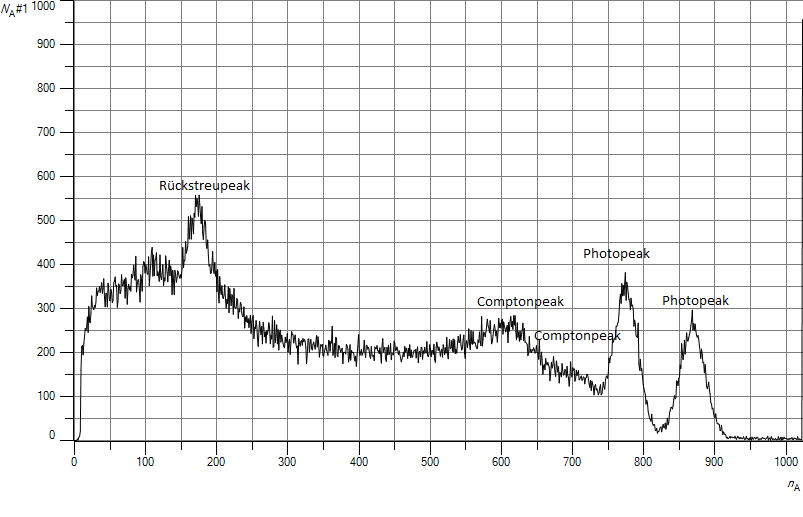
\includegraphics[width=0.8\textwidth]{bilder/aufgabe1/co60.png}\\
		\end{tabular}
		\caption{Impulshöhenspektrum von Co-60}
		\label{fig:co}
\end{figure}
\begin{figure}[H]
		\centering
		\begin{tabular}{@{}r@{}}
			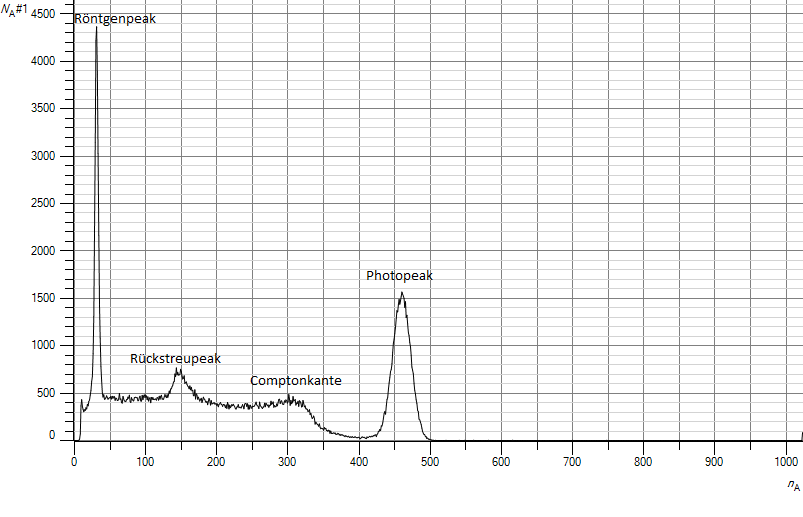
\includegraphics[width=0.8\textwidth]{bilder/aufgabe1/cs137.png}\\
		\end{tabular}
		\caption{Impulshöhenspektrum von Cs-137}
		\label{fig:cs}
\end{figure}
\begin{figure}[H]
		\centering
		\begin{tabular}{@{}r@{}}
			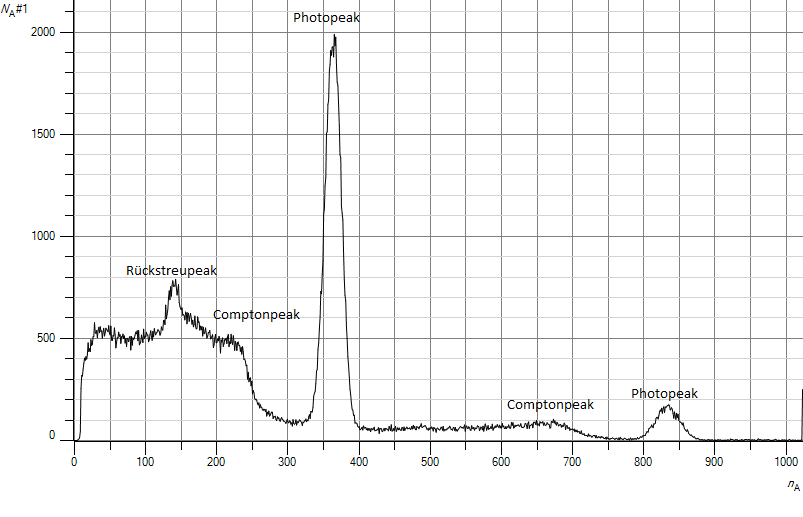
\includegraphics[width=0.8\textwidth]{bilder/aufgabe1/na22.png}\\
		\end{tabular}
		\caption{Impulshöhenspektrum von Na-22}
		\label{fig:na}
\end{figure}
Um die Energien der Peaks zu berechnen, muss zuvor eine Energieskalierung durchgeführt werden, also wie viel Energie einem Kanal entspricht. Dies sollte laut Aufgabenblatt anhand des Photopeaks für Cs-137 vorgenommen werden.\\ \\
Zunächst wurde mittels Gauß-Anpassung die Lage des Maximums des Cs-137 Photopeaks bestimmt, der im Aufgabenblatt mit $\unit[662]{keV}$ angegeben war:
\begin{equation*}
\sigma=13 \quad \quad \mu=460 \quad \quad A_1=\unit[1568]{keV}
\end{equation*}
Das Maximum des Peaks befindet sich also im Kanal 460 im Eichpunkt $\unit[662]{keV}$. Die Kalibrierung (Energie/Kanal) ergibt sich aus:
\begin{equation*}
\Delta E = \frac{N_A}{\mu}=\frac{\unit[662]{keV}}{460}=\unit[1.44]{keV}
\end{equation*}
Nun können die Energien der Peaks (Photo-, Rückstreupeaks und Compton-Kanten) berechnet werden. Die Bestimmung der Lage von Maxima erfolgt wieder mit Gauß-Anpassung der Peaks durch. Bei der Berechnung der Energien müsste der zuvor bestimmte Skalierungsfaktor $\Delta E$ berücksichtigt werden:
\begin{equation*}
E=\Delta E \cdot n_{max}
\end{equation*}
wobei $n_{max}$ die Kanalnummer im Maximum des Peaks ist. Die Tabellen enthalten die Ergebnisse der Berechnungen und einen Vergleich mit den in der Vorbereitung berechneten theoretischen Werten.

\begin{table}[H]
\begin{tabular}{l|c|c|c|c}
	Art des Peaks & $n_{max}$ & $\Delta E$ (gem.) [keV] & $\Delta E$ (theo.) [keV] & Abweichung [$\%$] \\
	\hline
	Photopeak & 460 & 662.4 & 662.4 & Eichung\\
	Comptonpeak & 321 & 462.24 & 478 & 3.3\\
	Rückstreupeak & 149 & 214.56 & 184 & 16.61\\
	Röntgenpeak & 31 & 44.64 & 32 & 39.5\\
\end{tabular}
\caption{Energien der Peaks für Cs-137}
\end{table}

\begin{table}[H]
\begin{tabular}{l|c|c|c|c}
	Art des Peaks & $n_{max}$ & $\Delta E$ (gem.) [keV] & $\Delta E$ (theo.) [keV] & Abweichung [$\%$] \\
	\hline
	Photopeak (rechts) & 839 & 1208.16 & 1275 & 5.24\\
	Comptonpeak (rechts) & 678 & 976.32 & 1062 & 8.07\\
	Photopeak (links) & 365 & 525.6 & 511 & 2.86\\
	Comptonpeak (links) & 236 & 339.84 & 341 & 0.01\\
	Rückstreupeak & 146 & 210.24 & 213 & 1.3\\
\end{tabular}
\caption{Energien der Peaks für Na-22}
\end{table}

\begin{table}[H]
\begin{tabular}{l|c|c|c|c}
	Art des Peaks & $n_{max}$ & $\Delta E$ (gem.) [keV] & $\Delta E$ (theo.) [keV] & Abweichung [$\%$] \\
	\hline
	Photopeak (links) (mm) & 868 & 1249.92 & 1333 & 6.23\\
	Photopeak (rechts) (mm) & 774 & 1114.56 & 1173 & 4.98\\
	Comptonpeak (links) & 673 & 969.12 & 1119 & 13.39\\
	Comptonpeak (rechts) & 630 & 907.2 & 963 & 5.79\\
	Rückstreupeak & 175 & 252 & 214 & 17.76\\
\end{tabular}
\caption{Energien der Peaks für Co-60}
\end{table}
Im Allgemeinen stimmen die Messwerte gut mit den theoretischen Werten überein. Insbesondere bei Na-22 treten nur sehr geringe Abweichungen auf.\\ \\
Des weiteren sollte die Anzahl der zu einem Photopeak beitragenden Elektronen, also die Auflösung des Detektors, abgeschätzt werden. Dazu verwendet man die Beziehung aus der Vorbereitung:
\begin{equation*}
n=\left(\frac{E}{\Delta E}\right)^2
\end{equation*}
wobei $\Delta E$ die Halbwertbreite des Peaks ist. Für die Berechnung wird das Photopeak von Cs-137 verwendet. Die Halbwertsbreite einer gaußartigen Kurve entspricht dem $2 \sqrt{2 \ln 2}$-fachen der Standardabweichung:
\begin{equation*}
n=\left(\frac{\unit[622]{keV}}{\unit[2 \sqrt{2 \ln 2} \cdot 13]{keV}}\right)^2=\left(\frac{\unit[622]{keV}}{\unit[30.61]{keV}}\right)^2=412.91
\end{equation*}
Abschließend sollte die Linearität der Apparatur überprüft werden. Dazu verwenden wir Informationen aus den 3 gewonnenen Spektren und das Wissen, dass die Summe der Quantenenergien im Rückstreu- und Comptonpeak der Quantenenergie im Photopeak entsprechen soll.
\begin{table}[H]
\begin{tabular}{c|c|c|c}
	Spektrum von & Summe [keV] & Energie Photopeak [keV] & Abweichung [\%]\\
	\hline
	Cs-137 & 676.8 & 662.4 & 2.17\\
	Na-22 & 824 & 839 & 1.79\\
	C0-27 & 848 & 868 & 2.3\\
\end{tabular}
\end{table}
Die größte Abweichung beträgt $\unit[2.3]{\%}$ und ist somit so klein, dass die Apparatur in guter Näherung als linear angenommen werden kann. Mit diesen Abweichungen (in absoluten Beträgen zwischen $\unit[14.4-20]{keV}$) lassen sich auch die Abweichungen der Peak-Energien zurückführen.
\section{Bestimmung der Aktivität des Cs-137 Präparats}
Die Aktivität des Cs-137 Präparats, eigentlich die Zerfallsrate (also die zeitliche Änderung der noch nicht zerfallenen Atome), soll in diesem Versuchsteil bestimmt werden. Dazu verwendet man folgenden Sachverhalt:
\begin{equation*}
A=\frac{dN}{dt}=\frac{n}{p(E,d) \cdot (1-t) \cdot \lambda}=\frac{n}{w \cdot (1-t)}
\end{equation*}
wobei $n$ die Zählrate, $p$ die Nachweiswahrscheinlichkeit eines Quants, $t$ die Totzeit in $\%$ und $\lambda$ die Zerfallswahrscheinlichkeit sind. Die Nachweiswahrscheinlichkeit und Zerfallswahrscheinlichkeit fassen wir in einer Größe $w$ zusammen, die die Detektionswahrscheinlichkeit der Teilchen angibt, leicht aus Abbildung 4 aus der Vorbereitungshilfe abgelesen werden kann und  vom Abstand Präparat-Szintillator als auch von der Energie abhängt.\\
Der Versuch wurde für drei verschiedene Abstände Quelle-Szintillatorstirnfläche durchgeführt. Dabei zeigte das Programm CASSY die Totzeit t sowie die Zählrate n, welche zu Auswertungszwecken im Versuchsprotokoll festgehalten wurden. $w$ liest man aus der Tabelle in der Vorbereitungshilfe für den jeweiligen Abstand und für die Energie $\unit[662]{keV}$, die dem Photopeak von Cs-137 entspricht, ab.\\ \\
Tabelle \ref{tab:aufgabe2} fasst diese Information und die berechnete Aktivität zusammen.
\begin{table}[H]
\begin{tabular}{c|c|c|c||c}
	Abstand [cm] & w & Totzeit t & n [$s^{-1}$] & A [Bq]\\
	\hline
	2 & 0.023 & 0.16 & 2142.85 & 110913.56\\
	3 & 0.015 & 0.13 & 1682.25 & 128908.05\\
	4 & 0.008 & 0.8 & 1148.51 & 717818.75\\
\end{tabular}
\label{tab:aufgabe2}
\end{table}
Durch Mittelwertbildung erhält man für die Aktivität den gesuchten Ausgleichswert:
\begin{equation*}
A=\unit[319213.45]{Bq}=\unit[319.2]{kBq}
\end{equation*}
Mit zunehmendem Abstand $d$ nimmt auch der Wert der Aktivität zu, was keinen Sinn hat, denn die Zerfallsrate soll unabhängig vom Abstand sein und hängt nur von der Probe selbst ab.\\ \\
Auch entspricht der Ausgleichswert nicht gerade der Aktivität der im Labor vorhandenen Cs-137 Präparate mit jeweils $\unit[140]{kBq}$, $\unit[170]{kBq}$ und $\unit[270]{kBq}$ (Abweichung $\unit[18.2]{\%}$).
\section{Röntgenemission}
In diesem Versuchsteil geht es darum unbekannte Materialien mit höheren Ordnungszahlen $Z$ mithilfe einer Cs-137-Quelle zur Röntgenemission anzuregen und sie zu bestimmen.\\ \\
Impulshöhenspektren sollen aufgenommen und die Röntgenpeaks mit Gaussfit bestimmt werden. Zunächst werden Impulshöhenspektren von bekannten Elementen (Ba und Pb) aufgenommen und nach vorheriger Energiekalibration in ein $E-Z^2$-Diagramm aufgetragen. Durch Auftragung der Energien der unbekannten Elemente in das bestehende Diagramm und dem nach der Moseleyschen Gesetz erwarteten $E-Z^2$-Linearität, kann man die Ordnungszahl $Z$ der unbekannten Elemente, somit auch die Elemente selbst, bestimmen.\\ \\
Für Pb ergibt der Gaußfit der Röntgenlinie einen Peak bei 669, für Ba einen Peak bei 300. Anhand der gemittelten K-Röntgenlinie bei jeweils $\unit[74.2]{keV}$ und $\unit[32.1]{keV}$, führen wir die Energiekalibrierung durch:
\begin{gather*}
669 - 300 \quad \Rightarrow \quad \unit[74.2]{keV}-\unit[32.1]{keV}\\
1 \quad \Rightarrow \quad \unit[0.11]{keV}
\end{gather*}
\begin{figure}[H]
		\centering
		\begin{tabular}{@{}r@{}}
			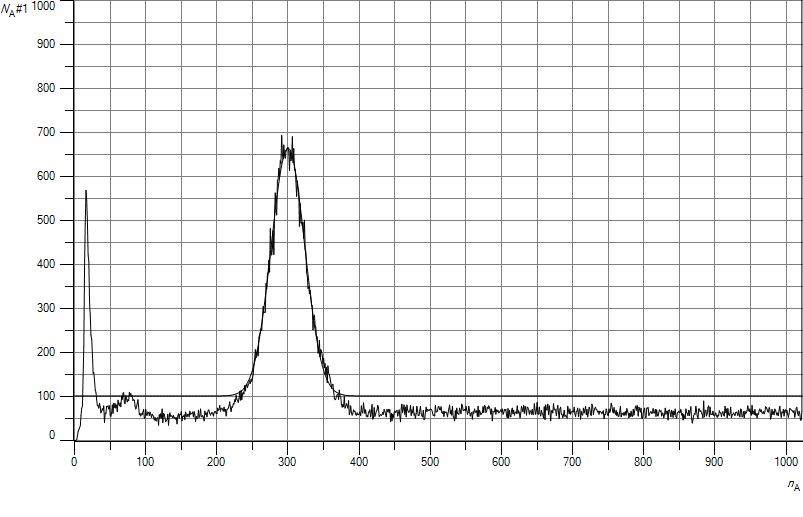
\includegraphics[width=0.8\textwidth]{bilder/aufgabe3/ba.png}\\
		\end{tabular}
		\caption{Impulshöhenspektrum von Ba}
\end{figure}
\begin{figure}[H]
		\centering
		\begin{tabular}{@{}r@{}}
			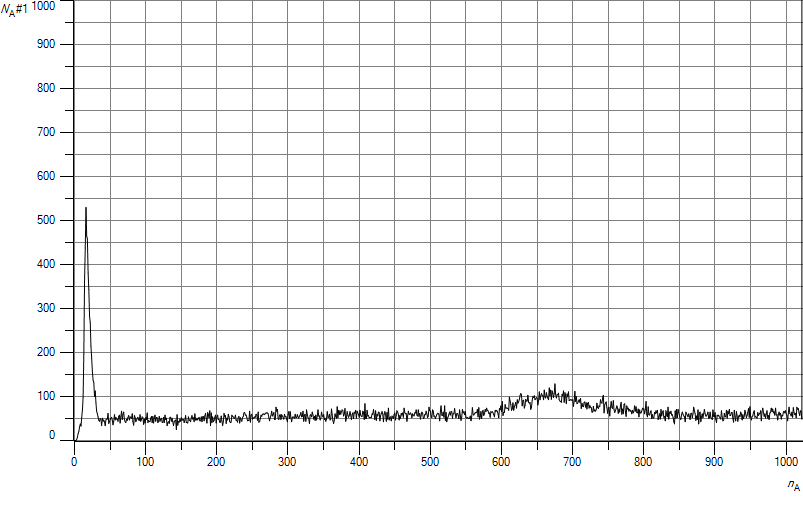
\includegraphics[width=0.8\textwidth]{bilder/aufgabe3/pb.png}\\
		\end{tabular}
		\caption{Impulshöhenspektrum von Pb}
\end{figure}
Nun können anhand der Peaks der Gaußfits der Röntgenlinie der unbekannten Elemente und der vorgenommenen Kalibrierung ihre Energien in der $K_{\alpha}$-Linie bestimmt werden und dann im $E-Z^2$-Diagramm aufgetragen werden:
\begin{table}[H]
\begin{tabular}{c|c}
	Element & Energie [keV]\\
	\hline
	A & 58.9\\
	B & 60.6\\
	C & -\\
\end{tabular}
\end{table}
Die nachfolgenden Abbildungen \ref{fig:aufgabe3a}-\ref{fig:aufgabe3c} zeigen die Röntgenpeaks und deren Gaußfits. Leider konnte beim Impulshöhenspektrum vom Element C kein Röntgenpeak identifiziert werden, sodass auch das Element selbst anhand der Energie im Peak nicht identifizieren werden kann.
\begin{figure}[H]
		\centering
		\begin{tabular}{@{}r@{}}
			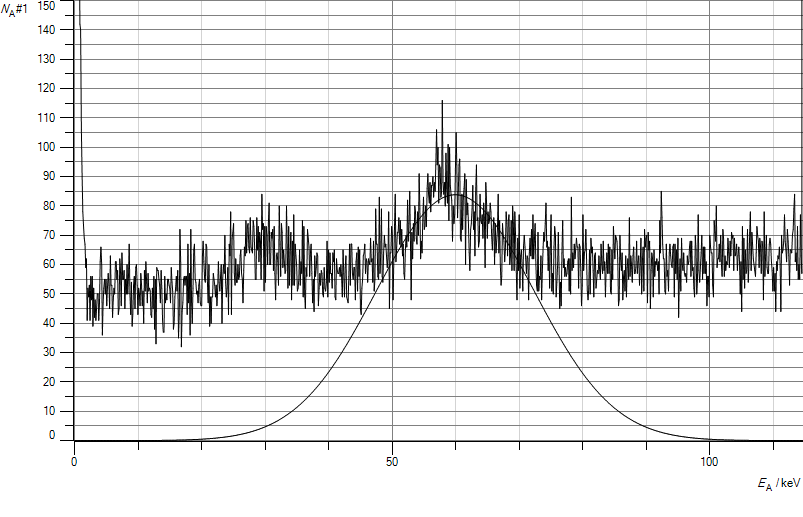
\includegraphics[width=0.45\textwidth]{bilder/aufgabe3/a.png}\\
		\end{tabular}
		\caption{Impulshöhenspektrum vom unbekannten Element A}
		\label{fig:aufgabe3a}
\end{figure}
\begin{figure}[H]
		\centering
		\begin{tabular}{@{}r@{}}
			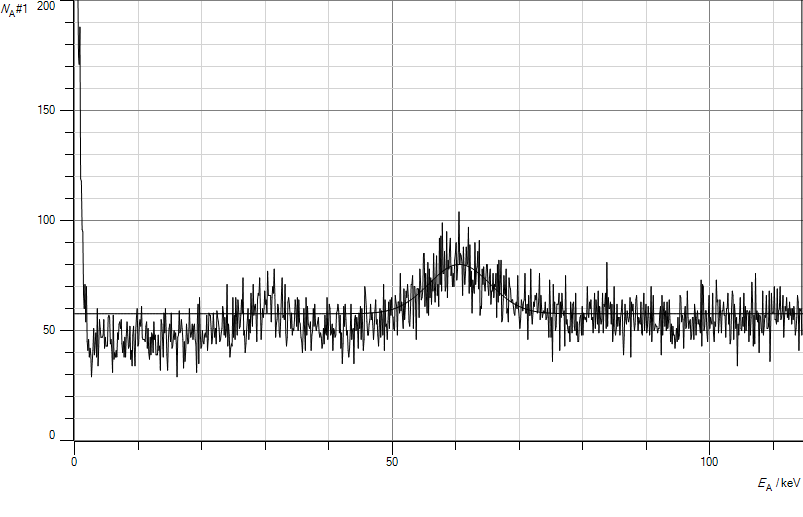
\includegraphics[width=0.45\textwidth]{bilder/aufgabe3/b.png}\\
		\end{tabular}
		\caption{Impulshöhenspektrum vom unbekannten Element B}
\end{figure}
\begin{figure}[H]
		\centering
		\begin{tabular}{@{}r@{}}
			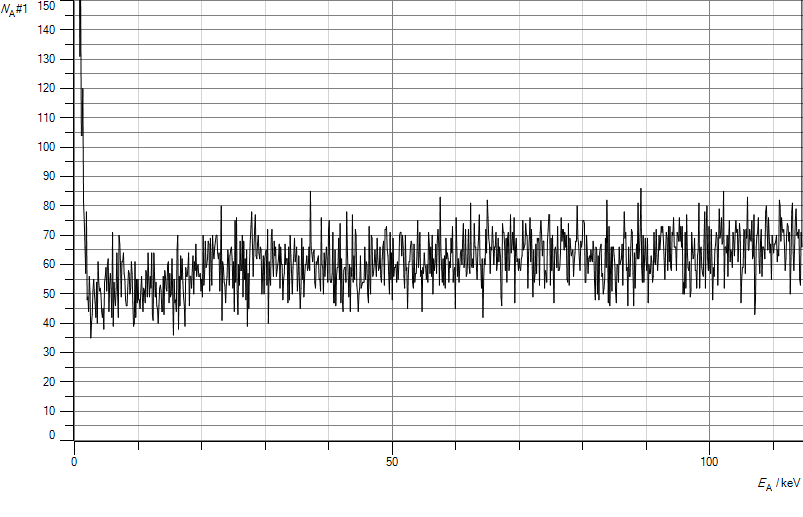
\includegraphics[width=0.45\textwidth]{bilder/aufgabe3/c.png}\\
		\end{tabular}
		\caption{Impulshöhenspektrum vom unbekannten Element C}
		\label{fig:aufgabe3c}
\end{figure}
Abbildung \ref{fig:aufgabe3ez} zeigt das $E-Z^2$-Diagramm. Anhand der Energien der unbekannten Elemente kann man die Ordnungszahl finden und daraus das Element bestimmen. Für das Element A findet man Ta (Tantalum), für das Element B W (Wolfram) heraus.
\begin{figure}[H]
		\centering
		\begin{tabular}{@{}r@{}}
			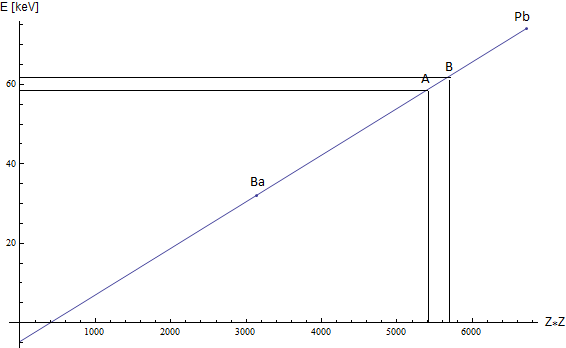
\includegraphics[width=0.8\textwidth]{bilder/aufgabe3/ez.png}\\
		\end{tabular}
		\caption{$E-Z^2$-Diagramm}
		\label{fig:aufgabe3ez}
\end{figure}
\section{Statistik}
\subsection{Statistische Verteilung von gemessenen Ereignisanzahlen bei häufig wiederholter Messung von Untergrundstrahlung}
Es wurden 150 Spektren (Spalten) im Vielkanalmodus mit 256 Kanälen (Zeilen) aufgenommen. Daraus sollten 2 Stichproben gebildet werden:
\begin{enumerate}
\item Stichprobe mit nur einem Teil des Spektrums, sodass der Mittelwert der 150 Summen der Zählraten ungefähr 3 beträgt. Hier wurden die Kanäle 79-94 gewählt.
\item Stichprobe mit allen Spektren
\end{enumerate}
\subsection{Mittelwert, Standardabweichung der Einzelmesswerte, Standardabweichung des Mittelwerts}
Mit den Formeln aus der Vorbereitung sollten für die beiden Stichproben der Mittelwert $x_m$, die Standardabweichung $x$ und Standardabweichung des Mittelwerts $s_m$ berechnet werden.
\begin{table}[H]
\begin{tabular}{c|c|c}
	& Stichprobe A & Stichprobe B\\
	\hline
	$x_m$ & 3.13 & 23.52\\
	$s$ & 1.69 & 4.85\\
	$s_{xm}$ & 0.14 & 0.40\\
	$\sqrt{x_m}$ & 1.77 & 4.85\\
\end{tabular}
\end{table}
\subsection{Darstellung der Häufigkeitsverteilung der Stichproben, Gauss- und Poissonverteilung}
Aus den oben ermittelten Daten (Mittelwert und Standardabweichung) sollten Häufigkeitsdiagramme (Histogramme) erstellt werden sowie die zugehörigen Fits der Poission- und Gauss-Verteilung.\\ \\
Man sieht, dass die Verteilung der Messwerte keiner der theoretischen Kurven entspricht.
\begin{figure}[H]
		\centering
		\begin{tabular}{@{}r@{}}
			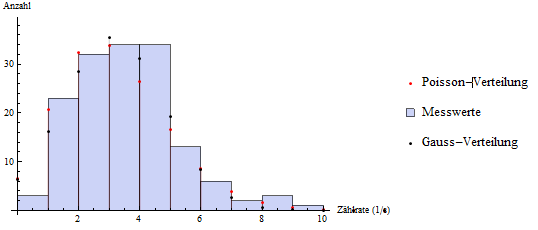
\includegraphics[width=0.9\textwidth]{bilder/Aufgabe4/probea.png}\\
		\end{tabular}
		\caption{Häufigkeitsverteilung für Stichprobe A}
		\label{fig:aufgabe4probaA}
\end{figure}
\begin{figure}[H]
		\centering
		\begin{tabular}{@{}r@{}}
			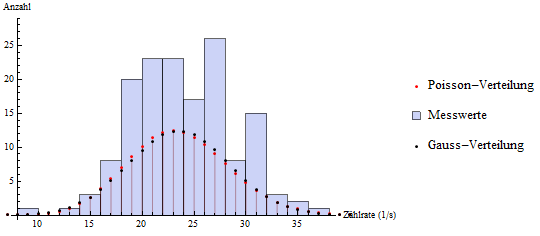
\includegraphics[width=0.9\textwidth]{bilder/aufgabe4/probeb.png}\\
		\end{tabular}
		\caption{Häufigkeitsverteilung für Stichprobe B}
		\label{fig:aufgabe4probaB}
\end{figure}
\end{document}